\chapter{Results and Analysis}
This chapter provides a graphical representation of the data acquired from conducting the tests designed in the last chapter. \todo{More overview}

\section{\acrlong{ht} Test}


\begin{figure}[h]
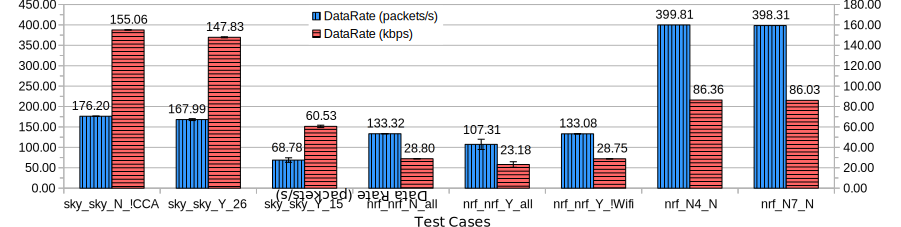
\includegraphics[width=\textwidth]{HT-dr}
\caption{Data Rate}
\end{figure}

\begin{figure}[h]
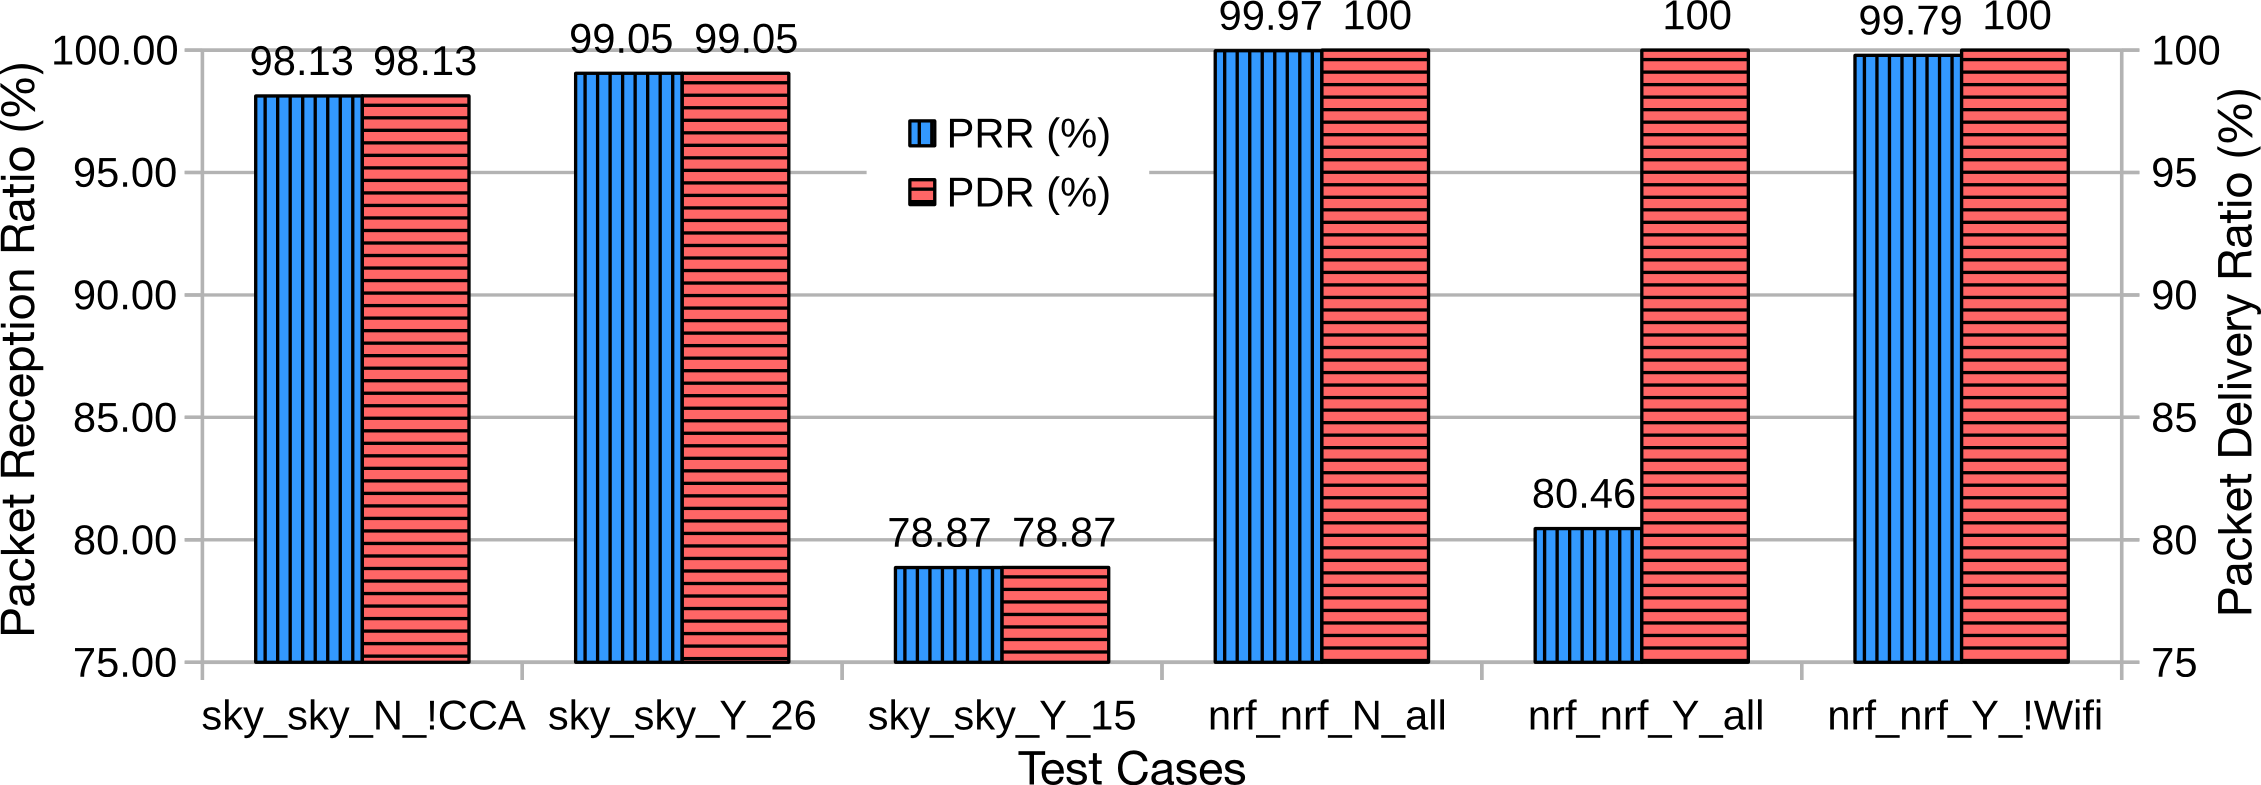
\includegraphics[width=\textwidth]{HT-r}
\caption{Reliability}
\end{figure}

\begin{figure}[h]
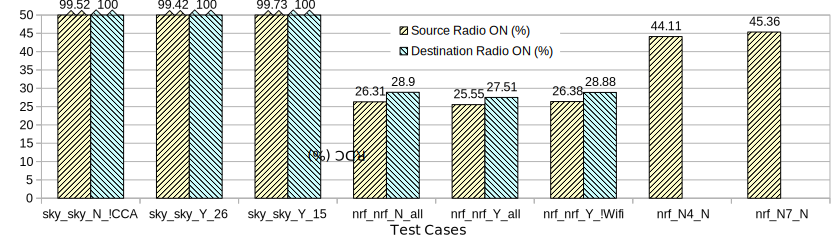
\includegraphics[width=\textwidth]{HT-ec}
\caption{Energy Consumption}
\end{figure}

\section{\acrlong{rr} Test}


\begin{figure}[h]
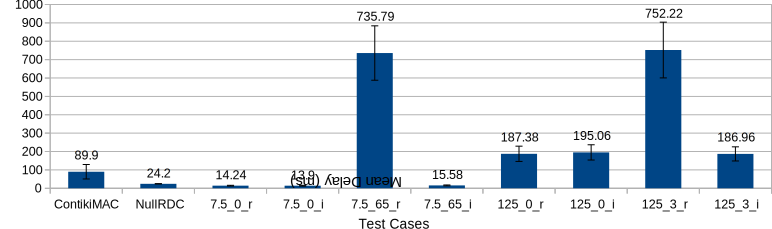
\includegraphics[width=\textwidth]{RR-l}
\caption{Latency}
\end{figure}

\begin{figure}[h]
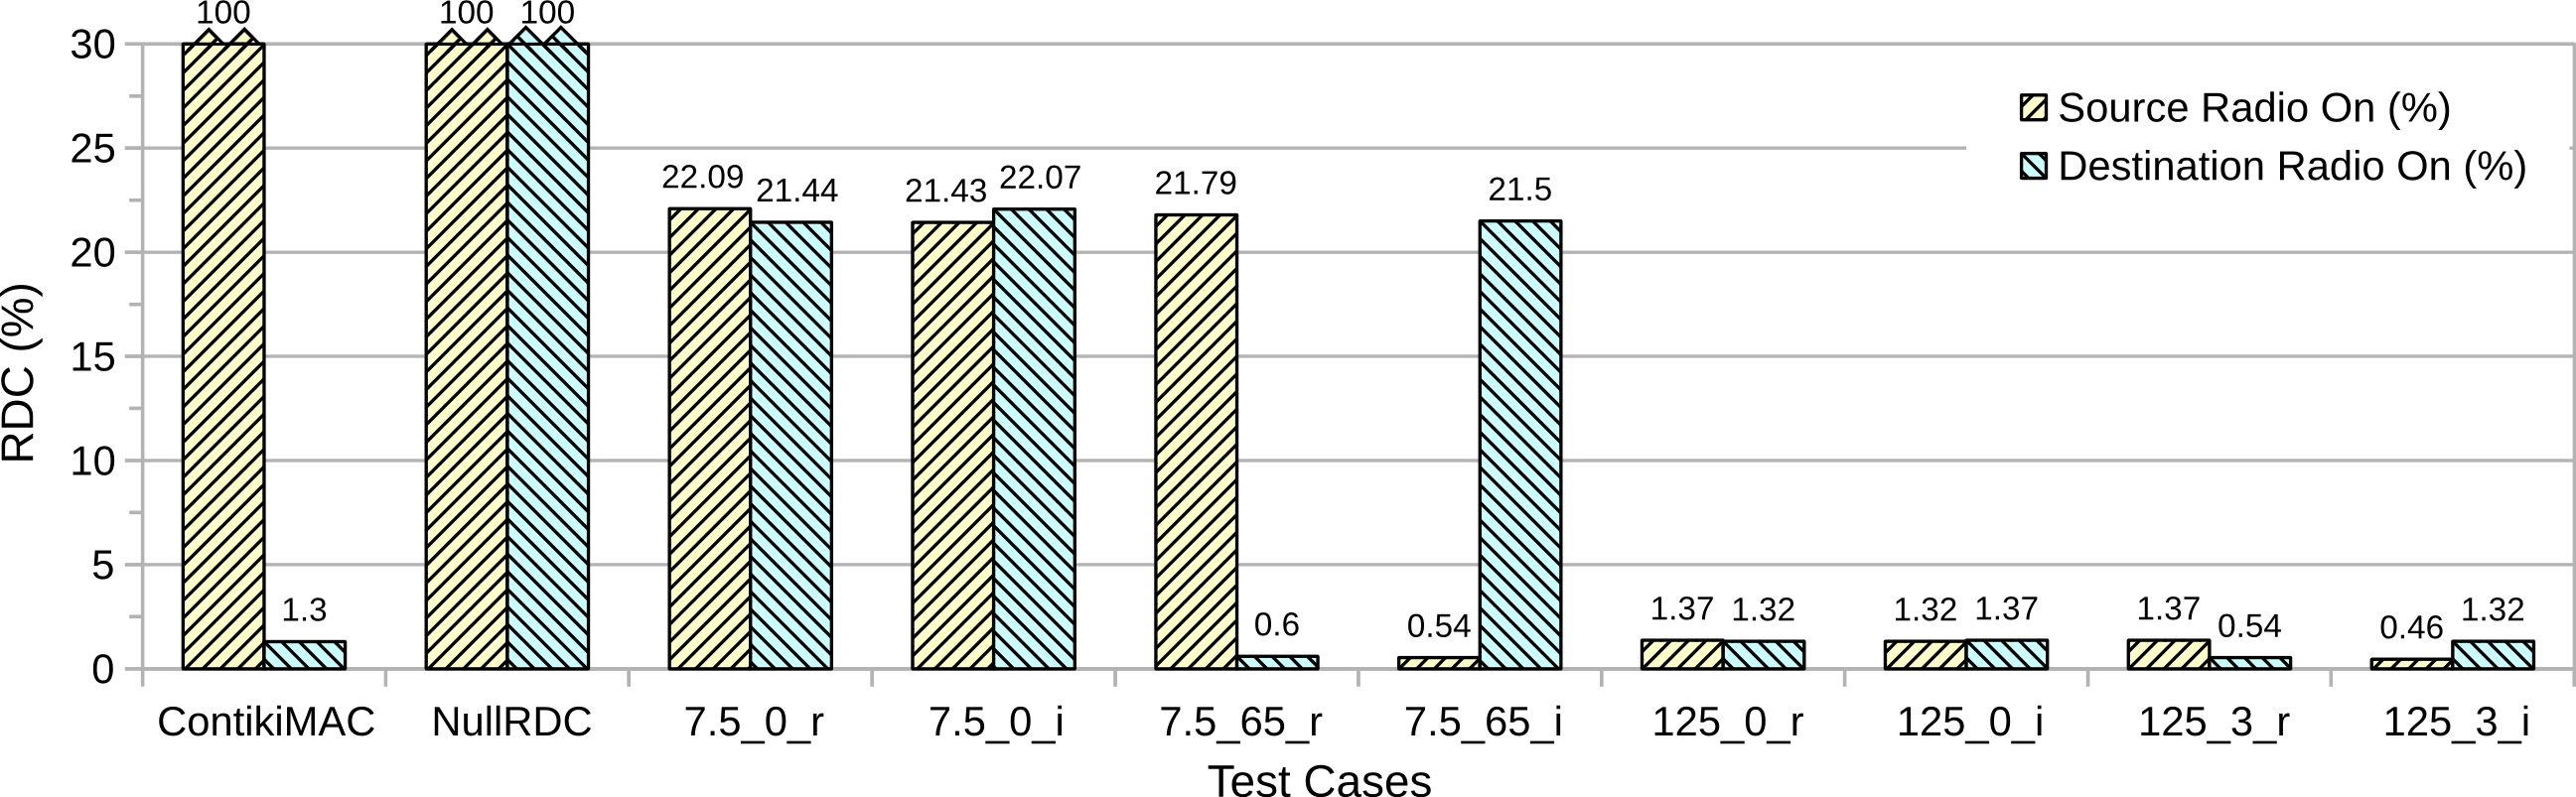
\includegraphics[width=\textwidth]{RR-ec}
\caption{Energy Consumption}
\end{figure}

\section{What we learnt}